\documentclass[oneside]{article}
\usepackage[paper=a4paper,margin=2cm,left=1cm]{geometry}
\usepackage{graphicx,tabularx}

\pagestyle{empty}

\begin{document}
    \begin{tabularx}{\linewidth}{| >{\centering\arraybackslash}X | >{\centering\arraybackslash}X |}
        \hline
        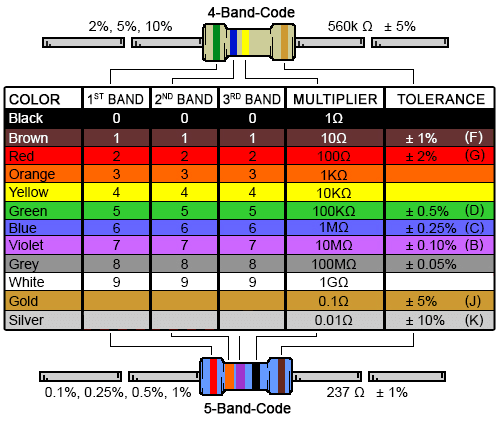
\includegraphics[height=5cm]{Extras/resistor_chart} & 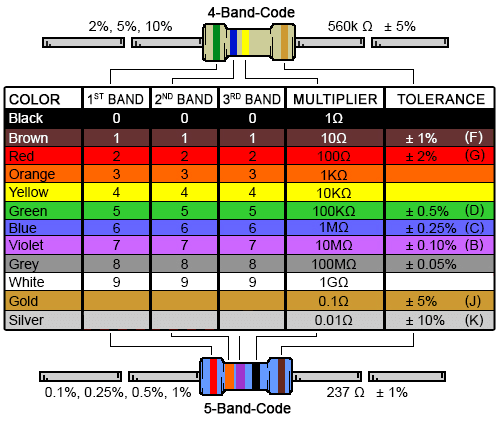
\includegraphics[height=5cm]{Extras/resistor_chart}\\\hline
        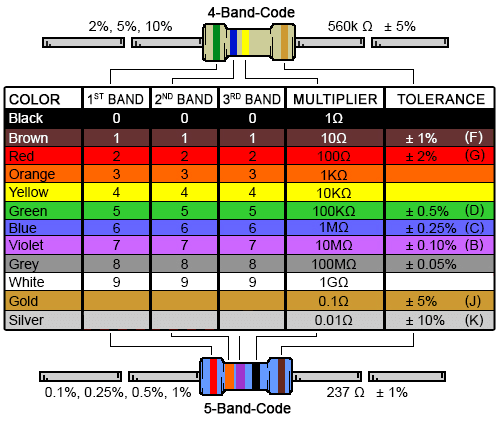
\includegraphics[height=5cm]{Extras/resistor_chart} & 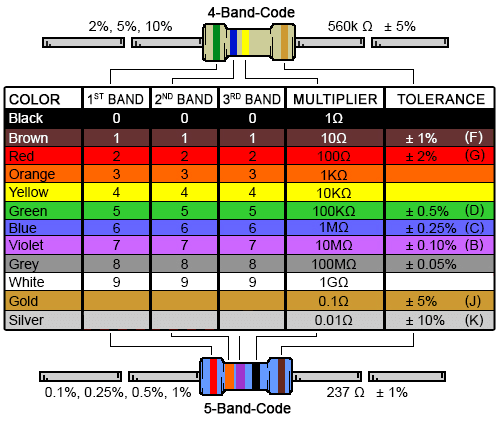
\includegraphics[height=5cm]{Extras/resistor_chart}\\\hline
        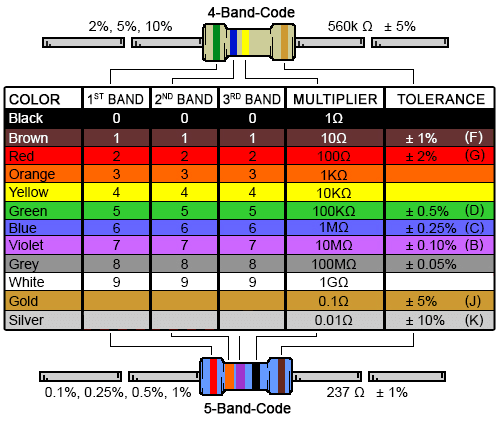
\includegraphics[height=5cm]{Extras/resistor_chart} & 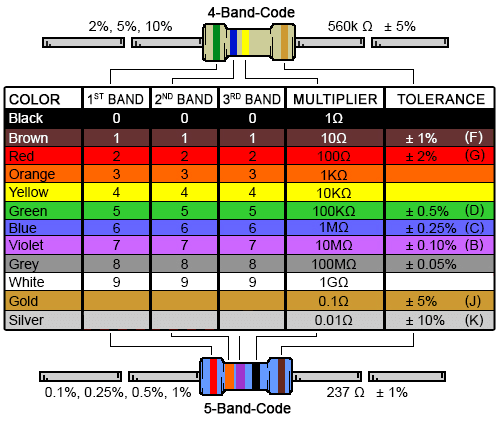
\includegraphics[height=5cm]{Extras/resistor_chart}\\\hline
        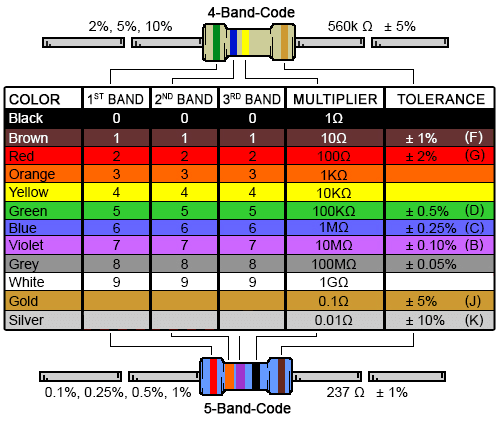
\includegraphics[height=5cm]{Extras/resistor_chart} & 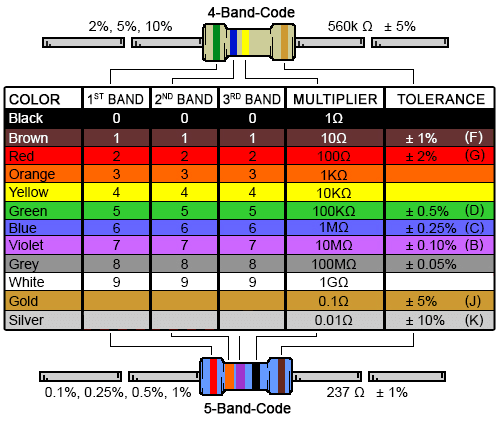
\includegraphics[height=5cm]{Extras/resistor_chart}\\\hline
        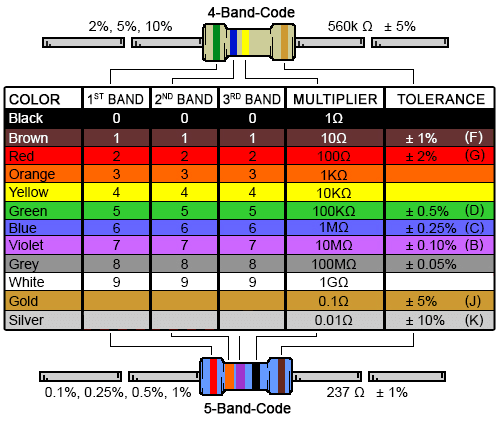
\includegraphics[height=5cm]{Extras/resistor_chart} & 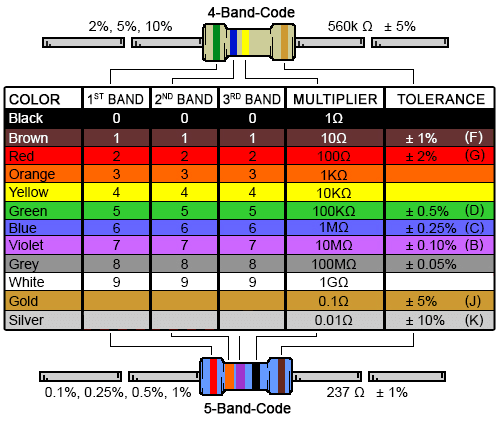
\includegraphics[height=5cm]{Extras/resistor_chart}\\\hline
    \end{tabularx}
\end{document}
